\documentclass{scrartcl}\usepackage[]{graphicx}\usepackage[]{color}
%% maxwidth is the original width if it is less than linewidth
%% otherwise use linewidth (to make sure the graphics do not exceed the margin)
\makeatletter
\def\maxwidth{ %
  \ifdim\Gin@nat@width>\linewidth
    \linewidth
  \else
    \Gin@nat@width
  \fi
}
\makeatother

\definecolor{fgcolor}{rgb}{0.345, 0.345, 0.345}
\newcommand{\hlnum}[1]{\textcolor[rgb]{0.686,0.059,0.569}{#1}}%
\newcommand{\hlstr}[1]{\textcolor[rgb]{0.192,0.494,0.8}{#1}}%
\newcommand{\hlcom}[1]{\textcolor[rgb]{0.678,0.584,0.686}{\textit{#1}}}%
\newcommand{\hlopt}[1]{\textcolor[rgb]{0,0,0}{#1}}%
\newcommand{\hlstd}[1]{\textcolor[rgb]{0.345,0.345,0.345}{#1}}%
\newcommand{\hlkwa}[1]{\textcolor[rgb]{0.161,0.373,0.58}{\textbf{#1}}}%
\newcommand{\hlkwb}[1]{\textcolor[rgb]{0.69,0.353,0.396}{#1}}%
\newcommand{\hlkwc}[1]{\textcolor[rgb]{0.333,0.667,0.333}{#1}}%
\newcommand{\hlkwd}[1]{\textcolor[rgb]{0.737,0.353,0.396}{\textbf{#1}}}%
\let\hlipl\hlkwb

\usepackage{framed}
\makeatletter
\newenvironment{kframe}{%
 \def\at@end@of@kframe{}%
 \ifinner\ifhmode%
  \def\at@end@of@kframe{\end{minipage}}%
  \begin{minipage}{\columnwidth}%
 \fi\fi%
 \def\FrameCommand##1{\hskip\@totalleftmargin \hskip-\fboxsep
 \colorbox{shadecolor}{##1}\hskip-\fboxsep
     % There is no \\@totalrightmargin, so:
     \hskip-\linewidth \hskip-\@totalleftmargin \hskip\columnwidth}%
 \MakeFramed {\advance\hsize-\width
   \@totalleftmargin\z@ \linewidth\hsize
   \@setminipage}}%
 {\par\unskip\endMakeFramed%
 \at@end@of@kframe}
\makeatother

\definecolor{shadecolor}{rgb}{.97, .97, .97}
\definecolor{messagecolor}{rgb}{0, 0, 0}
\definecolor{warningcolor}{rgb}{1, 0, 1}
\definecolor{errorcolor}{rgb}{1, 0, 0}
\newenvironment{knitrout}{}{} % an empty environment to be redefined in TeX

\usepackage{alltt}
\author{Konrad Medicus, Fabian Oberreiter,Tobias Hilgart}

\usepackage{babel,amsmath, amsthm}
\usepackage{hyperref}
\hypersetup{
    colorlinks=true, %set true if you want colored links
    linktoc=all,     %set to all if you want both sections and subsections linked
    linkcolor=blue,  %choose some color if you want links to stand out
}
\IfFileExists{upquote.sty}{\usepackage{upquote}}{}
\begin{document}

\title{QAD-Package}

\maketitle

\section{Introduction}

The QAD-\textit{'Quantification of Asymmetric Dependence'} package introduces a copula-based dependency measure capable of detecting and depicting asymmetry.\\
Dependency measures such as the various correlations are not applicable to measure asymmetric dependence. Using copulae one can 'measure' the distance of a given copula to independence (dependency measure $\zeta_1$; Trutschnig, 2011) and fulfill all requirements for an asymmetric dependency measure, such as invariant under scale changes, 1 iff $Y$ is a function of $X$, 0 iff independent etc.\\
However, when one works with samples -- observations $(x_1,y_1),\dots,(x_n,y_n)$ -- the true distribution they are drawn from is generally unknown, and so is the underlying copula.\\
Thus there is a need to find a 'good estimate' for said copula in the sense, that it gives a good estimate of the dependency measure.\\
However, in said measure, the 'known' approximation called \textit{empirical copula} does not provide a good estimate. This is why the package introduces a 'smooth aggregation' of the empirical copula, called \textit{empirical checkerboard copula}, that does provide a good estimates and enables the user to estimate the (asymmetric) dependence from a sample by computing it.

\section{Background}
The mathematics behind the QAD-package cover parts of basic statistics as well as new research done in the field. The following is supposed to give a very general idea of the mathematics used behind the QAD-package and is not detailing the construction of the underlying objects and functions.\\\\
A (two dimensional) copula is a distribution function from $[0,1]^2 \to [0,1]$ which has uniform marginal distributions. Sklar's theorem states that for any pair of random variables, there exists a copula that can map the values of the individual (marginal) distributions back to the value of the joint distribution. Thus, copulae connect the marginal distributions to the joint distribution. 
Similarly to the empirical distribution function, we can approximate the underlying copula with the empirical copula. As a mere aggregation does not result in some desired convergence properties, the empirical checkerboard copula (introduced in Griessenberger, 2018) is computed, which does satisfy these properties. 
This empirical checkerboard copula is then used to calculate a 'distance' (the $D_1$-metric; introduced in Trutschnig, 2011) to the product copula, which is the copula corresponding to two independent random variables, and thereby the dependence is measured.
Due to the computation process not being symmetrical, the two dependence values do not have to be the equal - there can be an asymmetry in the data -- the difference of these values is the asymmetry measure

\section{qad}

The qad-function does exactly that: From a given data frame containing a bivariate sample, on column per variable, it calculates the empirical checkerboard copula and computes the dependency measure, thus quantifying the asymmetric dependence of two random variables $X$ and $Y$.\\
In the example below, we calculate the dependence between a sample drawn from uniform distributed random variable $X$ and the sine of this sample $Y$. We expect $Y$ to be strongly dependent on $X$ and less so the other way around. This is because $Y$ is directly computed from $X$ using a non-bijective function.

\subsection{Example I}


\begin{knitrout}
\definecolor{shadecolor}{rgb}{0.969, 0.969, 0.969}\color{fgcolor}\begin{kframe}
\begin{alltt}
\hlstd{n} \hlkwb{=} \hlnum{300}
\hlstd{x} \hlkwb{=} \hlkwd{runif}\hlstd{(n,}\hlnum{0}\hlstd{,}\hlnum{30}\hlstd{)}
\hlstd{y} \hlkwb{=} \hlkwd{sin}\hlstd{(x)}
\hlstd{df} \hlkwb{=} \hlkwd{data.frame}\hlstd{(x,y)}
\hlstd{model} \hlkwb{=} \hlkwd{qad}\hlstd{(df,} \hlkwc{print} \hlstd{=} \hlnum{FALSE}\hlstd{,} \hlkwc{permutation} \hlstd{=} \hlnum{TRUE}\hlstd{)}
\hlstd{model}\hlopt{$}\hlstd{results}
\end{alltt}
\begin{verbatim}
##                        coef p.values
## 1        q(x1,x2) 0.7263205      0.0
## 2        q(x2,x1) 0.2269512      0.1
## 3 mean.dependence 0.4766358      0.0
## 4 asymmetry       0.4993693      0.0
\end{verbatim}
\end{kframe}
\end{knitrout}
\noindent
Indeed, we see that $q(x1,x2)$, meassuring how dependent $Y$ is on $X$, is much higher than $q(x2,x1)$. This is a simple example of two asymmetrically dependet random variables.\\\\
A permutated p-test can be performed to test for independence, as has been done in the example above. In this case, with a significance level of 5\%, we have to reject the nullhypothesis of independence for $q(x1,x2)$, but cannot do so for $q(x2,x1)$.\\
Such a permutated p-test is computed in the following way: From the original two samples $x_1,\ldots,x_n$ and $y_1,\ldots,y_n$, we take the doubled sample\\ $(x_1,y_1),\ldots,(x_n,y_n),(y_1,x_1),\ldots(y_n,x_n)$. From it we draw $n$ observations, calculate the qad value and check wether the calculated value is at least as big as the one of the original sample. We repeat this a number $R$ amount of times (R can be set with the argument nperm) and the fraction of runs where this is the case is our p-value.\\
To view the results of the qad-function one can use summary function on a qad-object. With pairwise.qad, one can calculate the qad-value for each pair of columns in a given data frame. The function Heatmap.qad visualizes these results nicely.

\subsection{Example II}
This small example illustrates how pairwise.qad can be used to look for pairwise dependencies in a multivariat sample. We use the attitude data set, which shows the proportion of favourable responses to each of 7 questions for employees in 30 departments. We calculate the qad values and corresponding p-values. Significant result are marked with \textit{*} in the heatmap.
\begin{knitrout}
\definecolor{shadecolor}{rgb}{0.969, 0.969, 0.969}\color{fgcolor}\begin{kframe}
\begin{alltt}
  \hlcom{#load attitude dataset}
  \hlstd{att} \hlkwb{=} \hlstd{attitude}
  \hlstd{model} \hlkwb{=} \hlkwd{pairwise.qad}\hlstd{(att,} \hlkwc{permutation} \hlstd{=} \hlnum{TRUE}\hlstd{)}
  \hlkwd{heatmap.qad}\hlstd{(model,} \hlkwc{significance} \hlstd{=} \hlnum{TRUE}\hlstd{)}
\end{alltt}
\end{kframe}
\end{knitrout}



\begin{knitrout}
\definecolor{shadecolor}{rgb}{0.969, 0.969, 0.969}\color{fgcolor}
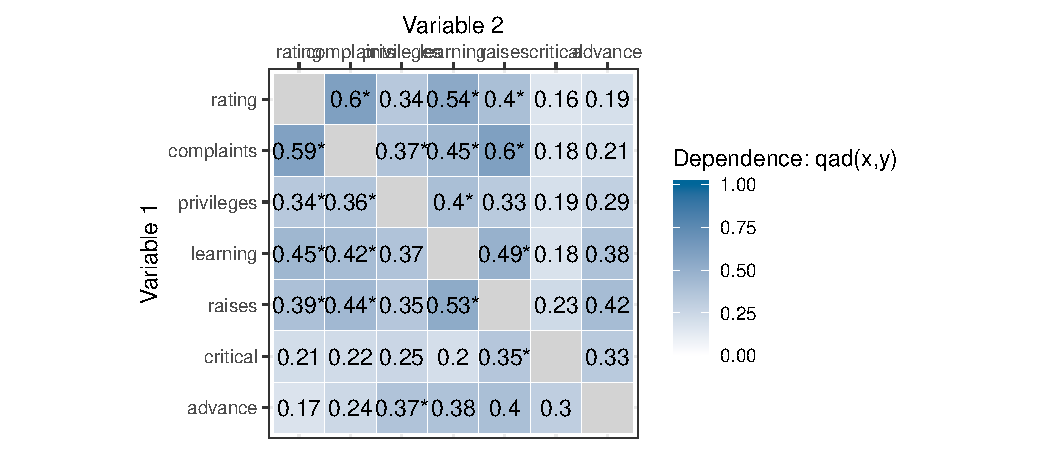
\includegraphics[width=\maxwidth]{figure/unnamed-chunk-5-1} 

\end{knitrout}

\section{cci}

cci (conditional confidence interval) provides a confidence interval, conditional on the sample size, for the qad-measure of two independent random variables. Thus it can be used to test for independence. The default significance level is 95\% and one-sided as well as two sided tests can be performed.

\begin{knitrout}
\definecolor{shadecolor}{rgb}{0.969, 0.969, 0.969}\color{fgcolor}\begin{kframe}
\begin{alltt}
\hlstd{c} \hlkwb{=} \hlkwd{cci}\hlstd{(n,} \hlkwc{alternative} \hlstd{=} \hlstr{"one.sided"}\hlstd{)}

\hlstd{x} \hlkwb{=} \hlkwd{runif}\hlstd{(n,}\hlopt{-}\hlnum{2}\hlstd{,}\hlnum{4}\hlstd{)}
\hlstd{y} \hlkwb{=} \hlkwd{sin}\hlstd{(x}\hlopt{^}\hlnum{2}\hlstd{)}
\hlstd{df} \hlkwb{=} \hlkwd{data.frame}\hlstd{(x,y)}
\hlstd{model} \hlkwb{=} \hlkwd{qad}\hlstd{(df,}\hlkwc{print}\hlstd{=}\hlnum{FALSE}\hlstd{)}

\hlkwa{if}\hlstd{(}\hlkwd{coef}\hlstd{(model,} \hlkwc{select} \hlstd{=} \hlstr{'q(x1,x2)'}\hlstd{)} \hlopt \hlstd{c)\{}
 \hlkwd{print}\hlstd{(}\hlstr{'Accept H0'}\hlstd{)}
\hlstd{\}}\hlkwa{else}\hlstd{\{}
 \hlkwd{print}\hlstd{(}\hlstr{'Reject H0'}\hlstd{)}
\hlstd{\}}
\end{alltt}
\begin{verbatim}
## [1] "Reject H0"
\end{verbatim}
\end{kframe}
\end{knitrout}

\section{Additional Functionalty}

If one desires to calculate just the empirical copula (smoothing=FALSE) or the checkerboard aggregation (smoothing=TRUE), one can do so by plugging data frame with bivariate sample into the emp\_ c\_ copula()-function. The resulting mass/density matrix can be plotted via plot\_ density.\\
Alternatively, calling the plot-function on a qad-object directly plots its mass matrix (from the checkerboard aggregation), one can also add the sample points and retransform from the copula into the original data setting.\\
Using the conditional probabilities, with the predict command on a qad-object, one gets the probabilities to land in certain intervals, given either certain $x$ or $y$ values (after specifying which are given). One can manually set the number of intervals, into which the range of the other random variable is splitted.

\subsection{Example III}
In this example we call plot() on a qad model. This visualizes the empirical checkerboard copula used to calculate the dependency meassure. The value of the blue rectangle in the plot give as an estimation of the conditional probability resulting in a value in the y-range of the rectangle, given that the x-value lies in the x-range.
\begin{knitrout}
\definecolor{shadecolor}{rgb}{0.969, 0.969, 0.969}\color{fgcolor}\begin{kframe}
\begin{alltt}
\hlkwd{set.seed}\hlstd{(}\hlnum{2017}\hlstd{)}
\hlstd{x} \hlkwb{=} \hlkwd{rnorm}\hlstd{(}\hlnum{50}\hlstd{,}\hlnum{1}\hlstd{,}\hlnum{2}\hlstd{)}
\hlstd{y} \hlkwb{=} \hlstd{x}\hlopt{^}\hlnum{2} \hlopt{+} \hlkwd{rnorm}\hlstd{(}\hlnum{50}\hlstd{,}\hlnum{0}\hlstd{,}\hlnum{1}\hlstd{)}
\hlstd{df} \hlkwb{=} \hlkwd{data.frame}\hlstd{(x,y)}

\hlstd{model} \hlkwb{=} \hlkwd{qad}\hlstd{(df,}\hlkwc{print}\hlstd{=}\hlnum{FALSE}\hlstd{)}
\hlkwd{plot}\hlstd{(model,} \hlkwc{copula} \hlstd{=} \hlnum{FALSE}\hlstd{)}
\end{alltt}
\end{kframe}
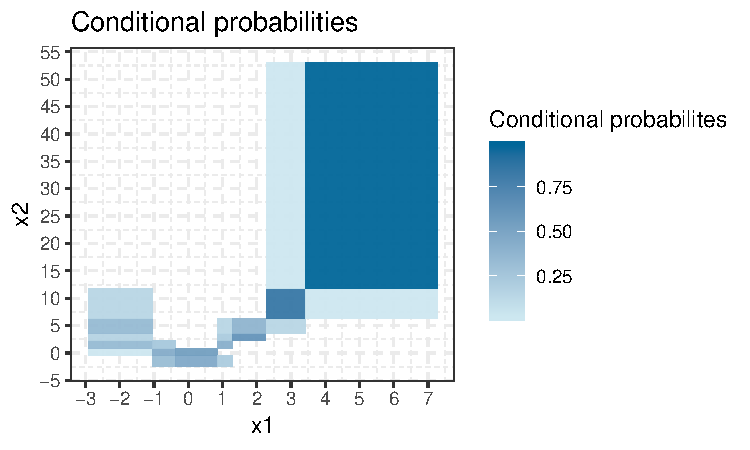
\includegraphics[width=\maxwidth]{figure/unnamed-chunk-7-1} 

\end{knitrout}

\subsection{Example IV}
The next example shows the call and output of the predict function. It shows the conditional probabilities to end up with $y$-value in the listed intervals for all the given values (-1 to 3).
\begin{knitrout}
\definecolor{shadecolor}{rgb}{0.969, 0.969, 0.969}\color{fgcolor}\begin{kframe}
\begin{alltt}
\hlkwd{predict}\hlstd{(model,} \hlkwc{values} \hlstd{=} \hlkwd{c}\hlstd{(}\hlopt{-}\hlnum{1}\hlstd{,}\hlnum{0}\hlstd{,}\hlnum{1}\hlstd{,}\hlnum{2}\hlstd{,}\hlnum{3}\hlstd{),} \hlkwc{conditioned} \hlstd{=} \hlstr{"x1"}\hlstd{,}
        \hlkwc{nr_intervals} \hlstd{=} \hlnum{5}\hlstd{)}
\end{alltt}
\begin{verbatim}
##    (-2.46,-0.1] (-0.1,1.85] (1.85,3.98] (3.98,10.22] (10.22,52.96]
## -1        0.496       0.456       0.048        0.000         0.000
## 0         0.676       0.324       0.000        0.000         0.000
## 1         0.220       0.336       0.332        0.112         0.000
## 2         0.000       0.000       0.696        0.304         0.000
## 3         0.000       0.000       0.028        0.616         0.356
\end{verbatim}
\end{kframe}
\end{knitrout}

\section*{References}	
\url{https://arxiv.org/ftp/arxiv/papers/1902/1902.00203.pdf} \\
\url{https://cran.r-project.org/web/packages/qad/qad.pdf} \\
\url{http://www.trutschnig.net/slides_qad_handout.pdf} \\
\url{http://www.trutschnig.net/qad_maths.pdf} 

\end{document}
